%----------------------------------------------------------------------------------------
%	METODE
%----------------------------------------------------------------------------------------
\section*{TINJAUAN PUSTAKA}

\subsection*{\textit{Biodiversity Information}}

\textit{Biodiversity} atau keanekaragaman hayati mengacu pada upaya untuk mempelajari kehidupan di bumi. Keanekaragaman yang dipelajari meliputi bidang molekul, organisme dan ekologi (Sarkar 2007). \textit{Biodiversity information} (BI) merupakan upaya untuk membuat sumber informasi keanekaragaman hayati global tersedia dalam format digital yang efisien, dan untuk mengembangkan alat yang efektif dalam menganalisis dan memahami data tersebut (\citeauthor{GILLMANE2009} \cite*{GILLMANE2009}).  Salah satu tantangan utama dalam BI adalah untuk memberikan data pengetahuan mengenai keanekaragaman hayati dengan cepat, dengan pengetahuan tersebut dapat dibangun sistem keanekaragaman hayati yang terpadu (\citeauthor{GILLMANE2009} \cite*{GILLMANE2009}).

\subsection*{Tumbuhan Obat}

Sampai tahun 2001 Laboratorium Konservasi Tumbuhan, Fakultas Kehutanan IPB telah mendata dari berbagai laporan penelitian dan literatur tidak kurang dari 2039 spesies tumbuhan obat yang berasal dari hutan Indonesia. Berdasarkan keanekaragamannya, tumbuhan obat dapat dikelompokkan berdasarkan familinya, formasi hutan, habitus, dan bagian tumbuhan yang dapat digunakan sebagai obat (\citeauthor{ZUHUD2008} \cite*{ZUHUD2008}). Bagian-bagian tumbuhan yang dapat digunakan sebagai obat sangat bervariasi mulai dari daun muda atau pucuk, buah, batang, kulit, getah, umbi dan akar (\citeauthor{HAMZARI2008} \cite*{HAMZARI2008}).

\subsection*{Ontologi}

Ontologi adalah suatu metode yang digunakan untuk merepresentasikan pengetahuan yang mendefinisikan hubungan dan klasifikasi dari pengetahuan tertentu (\citeauthor{JEPSEN2010} \cite*{JEPSEN2010}). Seperti pemrograman berorientasi objek, ontologi juga menggunakan kelas dan \textit{instance} dalam merepresentasikan pengetahuan. Namun, ontologi dengan pemrograman berorientasi objek berbeda dalam implementasinya. Pada pemrograman berorientasi objek \textit{instance} merupakan contoh nyata dari kelas tersebut. Pada ontologi, \textit{instance} bermakna anggota suatu domain tertentu (\citeauthor{JEPSEN2010} \cite*{JEPSEN2010}).

\subsection*{\textit{Gene Ontology} (GO)}

\textit{Gene ontology} (GO) dikembangkan oleh Gene Ontology Consortium untuk memberikan informasi mengenai gen yang lebih dinamis, terkontrol dan memiliki aturan yang sama. GO memiliki tiga komponen ontologi yaitu \textit{Biological Processes}, \textit{Cellular Components} dan \textit{Molecular Function}.  \textit{Biological processes}  mengacu gen atau \textit{gene product} yang berkontribusi pada suatu objek biologis. \textit{Molecular function} mengacu pada aktifitas biokimia yang terjadi pada \textit{gene product}. \textit{Cellular components} adalah tempat sel aktif yang berada di dalam \textit{gene product} (\citeauthor{ASHBURNERM2000} \cite*{ASHBURNERM2000}).

\subsection*{Web Semantik}

Web semantik adalah suatu \textit{framework} yangg memungkinkan data dan pengetahuan untuk dipublikasikan, membagi dan menggunakan kembali pengetahuan yang terdapat pada internet (\citeauthor{DINGL2005} \cite*{DINGL2005}). Web semantik adalah suatu \textit{graph} yang besar yang tersusun dari \textit{graph-graph} yang lebih kecil. (\citeauthor{SEGARAB2009} \cite*{SEGARAB2009}).

\subsection*{\textit{Resource Description Framework} (RDF)}

eXtensible Markup Language (XML) adalah suatu bahasa yang direpresentasikan dengan \textit{metadata}. XML merepresentasikan informasi agar dapat dengan mudah diakses oleh mesin. XML tidak menyediakan tag-tag tertentu, tetapi penggunanya dapat mendefiniskan tag secara mandiri. Namun, XML tidak dapat menunjukkan arti dari suatu data. RDF merupakan suatu bentuk dari data model. RDF mengadopsi sintaks-sintaks yang dimiliki oleh XML. Menurut Antoniou dan Hermalen (\cite*{ANTONIOUG2008}), RDF memiliki konsep dasar RDF yaitu \textit{resource}, \textit{properties}, dan \textit{statement}. \textit{Resource} adalah objek atau tentang sesuatu yang ingin diungkapkan. Beberapa contoh \textit{resource} seperti judul buku, pengarang, penerbit, orang dan sebagainya. Setiap \textit{resource} memiliki \textit{Universal Resource
Identifier} (URI). \textit{Properties} adalah deskripsi hubungan antar \textit{resource}, misalnya properti yang menghubungkan antara buku dengan penulisnya adalah “ditulis oleh”. \textit{Statement} adalah bentuk literal dari \textit{resource}, \textit{properties} dan nilainya. Menurut Raimbault (\cite*{RAIMBAULT2010})), statement disebut juga dengan triple model.

\begin{figure}[h!] % Gunakan \begin{figure*} untuk memasukkan Gambar
	\centering
	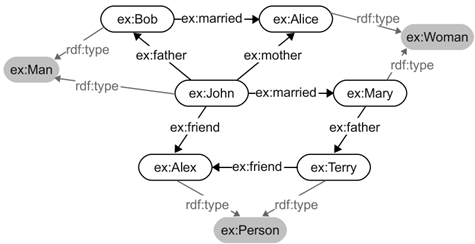
\includegraphics[width=200pt]{model_rdf_contoh_gb1.png}
	\caption{Contoh Model RDF}
	\label{fig:model_rdf}
\end{figure}

Gambar \ref{fig:model_rdf} menunjukkan contoh model RDF yang direpresentasikan dalam bentuk \textit{graph}.  Contoh \textit{statement} yang dapat dilihat dari Gambar \ref{fig:model_rdf} adalah John menikah dengan Mary.

\subsection*{\textit{Web Ontology Language} (OWL)}

\textit{Web Ontology Language} (OWL) adalah bahasa yang digunakan untuk membaca dan mendefinisikan kelas dan properti model RDF (\citeauthor{SEGARAB2009} \cite*{SEGARAB2009}). OWL merupakan bahasa yang kompleks. Oleh karena itu, OWL dibagi menjadi tiga sub bahasa berdasarkan tingkat kompleksitasnya, yaitu OWL-Lite, OWL DL dan OWL Full. OWL-Lite merupakan bentuk sub bahasa OWL yang paling sederhana. OWL DL memiliki fitur yang dapat digunakan untuk memaksimalkan penggunaan sistem \textit{reasoning} dan dapat menjamin kelengkapan informasi yang ingin didapat. OWL Full memberikan fitur yang membebaskan dalam mendeskripsikan sintaks RDF, tetapi tidak menjamin kelengkapan informasi yang didapat (He dan An 2011). OWL memiliki struktur data yang terdiri dari \textit{namespace} dan \textit{ontology head}. \textit{Namespace} digunakan untuk mengelompokkan \textit{identifier}. \textit{Ontology head} digunakan untuk mengumpulkan informasi metadata OWL yang digunakan (\citeauthor{HEG2010} \cite*{HEG2010}).

\subsection*{\textit{Simple Protocol and RDF Query Language} (SPARQL)}

\textit{Simple Protocol and RDF Query Language} (SPARQL) adalah bahasa \textit{query} yang digunakan untuk melakukan query data terhadap model RDF. Sama halnya dengan \textit{query} pada SQL, SPARQL juga digunakan untuk melakukan \textit{query} data-data yang diinginkan. Pembedanya, SQL melakukan \textit{query} pada \textit{database} yang terdiri dari satu atau beberapa tabel, sedangkan SPARQL melakukan \textit{query} pada data RDF yang berupa triple model (Segaran et al. \citeauthor{SEGARAB2009} \cite*{SEGARAB2009}). Berikut contoh sintaks SPARQL:
\\

PREFIX fb:$<$http://rdf.freebase.com/ns/$>$

SELECT ?who ?film

WHERE \{

?film fb:film.film.directed\_by ?who

?film fb:film.film.starring ?who

\}
\\

\textit{Query} dari SPARQL hampir sama seperti pada bahasa \textit{query} yang lain. Seperti sintaks SELECT, WHERE dan lainnya. Sintaks PREFIX digunakan untuk menyingkat alamat sumber dari data ontologi.

\subsection*{\textit{Semantic Web Object Oriented Design Methodology} (SW-OODM)}

\textit{Object Oriented Design Methodology} (OOMD) adalah metode yang digunakan untuk mengembangkan aplikasi web. Metode ini berguna untuk menangkap kebutuhan pengguna. Dengan adanya metode ini aktfitas pengembangan dapat dikontrol dengan baik (\citeauthor{FAROOQA2010} \cite*{FAROOQA2010}). SW-OODM merupakan metode pengembangan aplikasi web semantik yang merupakan pengembangan dari OOMD. SW-OODM meliputi aktivitas yang berguna untuk memformulasikan dan mendeskripsikan pengetahuan, sehingga aplikasi yang dibuat dapat dimengerti baik oleh mesin maupun oleh manusia (\citeauthor{FAROOQA2010} \cite*{FAROOQA2010}). Aktivitas yang terdapat di metode SW-OODM yaitu meliputi analysis phase dan design phase.Tahapan-tahapan yang berada dalam \textit{analysis phase} dikelompokan ke dalam empat model: \textit{preliminary web-ontology model}, \textit{information model}, \textit{user model}, dan \textit{operation model}. Sedangkan pada design phase dikelompokan menjadi enam unit: \textit{namely}, \textit{building component model}, \textit{building navigation model}, \textit{building operation partitioning model}, \textit{web ontology model} dan \textit{semantic web-page design} (Farooq et al. 2010).

